\documentclass[10pt,journal,compsoc]{IEEEtran}
% TNSE 官方模板走 Computer Society 模式（bare_jrnl_compsoc.tex，IEEEtran V1.8b）

% ==== packages ====
\usepackage[T1]{fontenc}
\usepackage[utf8]{inputenc}
\usepackage{amsmath,amssymb,amsfonts}
\usepackage{graphicx}
\usepackage{booktabs}
\usepackage{multirow}
\usepackage{algorithm}
\usepackage{algpseudocode}
\usepackage{xcolor}
\usepackage{tikz}
\usetikzlibrary{arrows.meta,positioning,fit,backgrounds}
\usepackage[colorlinks=true,linkcolor=blue,citecolor=blue,urlcolor=blue]{hyperref}
\usepackage{cleveref}
% 图表/公式引用统一为大写缩写格式：Fig. 1 / Table 1 / Eq. (7)
\crefname{figure}{Fig.}{Figs.}
\Crefname{figure}{Fig.}{Figs.}
\crefname{table}{Table}{Tables}
\Crefname{table}{Table}{Tables}
\crefname{equation}{Eq.}{Eqs.}
\Crefname{equation}{Eq.}{Eqs.}
\crefname{section}{Section}{Sections}
\Crefname{section}{Section}{Sections}
\creflabelformat{equation}{(#2#1#3)}

% ==== macros ====
\newcommand{\sysname}{SpaTE\xspace}
\usepackage{xspace}
% 审稿修改标记（定稿删除）
\newcommand{\todo}[1]{\textcolor{red}{[TODO: #1]}}
% 差异表勾叉符号
\newcommand{\cmark}{$\checkmark$}
\newcommand{\xmark}{$\times$}
% 定理环境（IEEEtran 内置支持）
\newtheorem{proposition}{Proposition}

\begin{document}

\title{\sysname: Learning-Based Traffic Engineering under Sparse Traffic
Observation in LEO Satellite Constellations}

\author{%
    Linhui~Wei,
    He~Ma,
    Yumei~Wang,~\IEEEmembership{Member,~IEEE,}
    and~Guangteng~Fan%
    \IEEEcompsocitemizethanks{%
        \IEEEcompsocthanksitem L. Wei and G. Fan are with the National
        Innovation Institute of Defense Technology, Academy of Military
        Science, Beijing, China (e-mail: weilinhui998@163.com;
        fanguangteng@163.com).%
        \IEEEcompsocthanksitem H. Ma and Y. Wang are with the School of
        Artificial Intelligence, Beijing University of Posts and
        Telecommunications, Beijing, China (e-mail: mahe@bupt.edu.cn;
        ymwang@bupt.edu.cn).%
        \IEEEcompsocthanksitem Manuscript received XXX; revised XXX.
        (Corresponding author: Guangteng Fan.)%
    }%
}

\markboth{IEEE Transactions on Network Science and Engineering}
{Wei \MakeLowercase{\textit{et al.}}: \sysname: Learning-Based Traffic Engineering under Sparse Traffic Observation in LEO Satellite Constellations}

% compsoc 模式：摘要与关键词包进 title-abstract-index 块
\IEEEtitleabstractindextext{%
\begin{abstract}
Low-Earth-orbit (LEO) satellite constellations require traffic
engineering (TE) that reacts quickly to changing topology and demand.
Existing learned TE systems achieve low online latency but assume a complete
traffic matrix, whereas telemetry and onboard-resource constraints allow a
constellation controller to meter only a fraction of demands at each epoch.
This paper presents \sysname, a sparse-aware TE system that allocates all
demands directly from incomplete observations, and rests on three ideas.
First, each unmeasured demand is represented by a learnable mask embedding,
so the model input separates ``not measured'' from ``no traffic'' instead of
fabricating a volume. Second, message passing over the path--link graph is
gated asymmetrically: unmeasured demands read link states but write nothing
into them, which provably keeps surrogate values out of the link
representation and out of every measured demand's allocation. Third, a
temporal encoder over recent sparse snapshots is fused with the spatial
representation by per-demand cross-attention, so history governs which
spatial evidence to trust where the current entry is missing. A
source-neighbor estimate additionally supplies the congestion signal for
optional deployment-time refinement without access to the ground-truth
matrix. On a 1{,}584-satellite Starlink constellation observed at ratios
from $2\%$ to $50\%$, \sysname{} decides in under $0.4$~s per snapshot,
realizes a maximum link utilization (MLU) of $1.64$--$1.89$, within
$1.19$--$1.37\times$ of the path-restricted linear-programming optimum, and
transfers to a one-third-scale constellation unchanged. Measured against
impute-then-optimize pipelines and a temporal baseline on zero-filled
input, which together test whether reconstructing the matrix or history
alone can substitute for explicit mask awareness, \sysname{} attains the
lower MLU in 15 to 16 of 25 matched trials, yet no pairwise comparison is
significant under a two-sided sign test. Ablations attribute a $6.7\%$ MLU
reduction at a $50\%$ observation ratio to end-to-end training and show the
source-neighbor estimate lowering median MLU from $2.30$ to $1.74$ against
zero filling, while the representation components trade places at the
sparsest ratios. We therefore report complete distributions over training
initializations, whose spread suffices to reverse rankings drawn from any
single aggregate score, and delimit where sparse-aware learning currently
helps.
\end{abstract}

\begin{IEEEkeywords}
LEO satellite constellation, traffic engineering, sparse traffic
measurement, maximum link utilization (MLU), graph neural networks.
\end{IEEEkeywords}}

\maketitle

\IEEEdisplaynontitleabstractindextext
\IEEEpeerreviewmaketitle

\IEEEraisesectionheading{\section{Introduction}\label{sec:intro}}

% 场景立意：卫星网络为何天然需要稀疏观测 TE → 三个挑战 → SpaTE 设计 →
% 诚实报告不同观测区间的结果。Fig. 1 恢复为稀疏观测场景图。

\IEEEPARstart{L}{ow-Earth-orbit} (LEO) satellite constellations are rapidly
scaling toward tens of thousands of satellites~\cite{handley2018,
bhattacherjee2019}. Their inter-satellite links (ISLs) carry
spatially concentrated and temporally varying traffic under limited
capacity~\cite{kassing2020}. Traffic engineering (TE), which
coordinates how each demand is split across candidate paths, is therefore
a key control primitive~\cite{jain2013,hong2018}. Classical
optimization can take minutes at constellation scale, whereas learned
allocators reduce online decision time to the sub-second range by moving
most computation offline~\cite{teal,dote,sate}.

Many learned TE systems nevertheless rely on a complete traffic matrix
at every control epoch. This assumption is particularly fragile in an LEO
constellation. Measuring every demand requires satellites to meter,
aggregate, and transmit fine-grained statistics through telemetry channels
that compete with user traffic for ISL and ground-station
bandwidth~\cite{kassing2020,michel2022}. It also consumes onboard
computation, storage, and power, while intermittent ground contacts
introduce unavoidable gaps; the expense of network-wide metering is the very
reason terrestrial operators have long inferred traffic matrices instead of
measuring them~\cite{vardi1996,zhang2003}. As illustrated in
\cref{fig:scenario}, only a subset of satellites may meter traffic at a
given epoch. The controller then receives a sparse traffic matrix but must
still allocate every demand. Efficient TE from sparse observations is thus
a natural operating mode for LEO networks, not merely a degraded version
of complete measurement.

\begin{figure}[t]
    \centering
    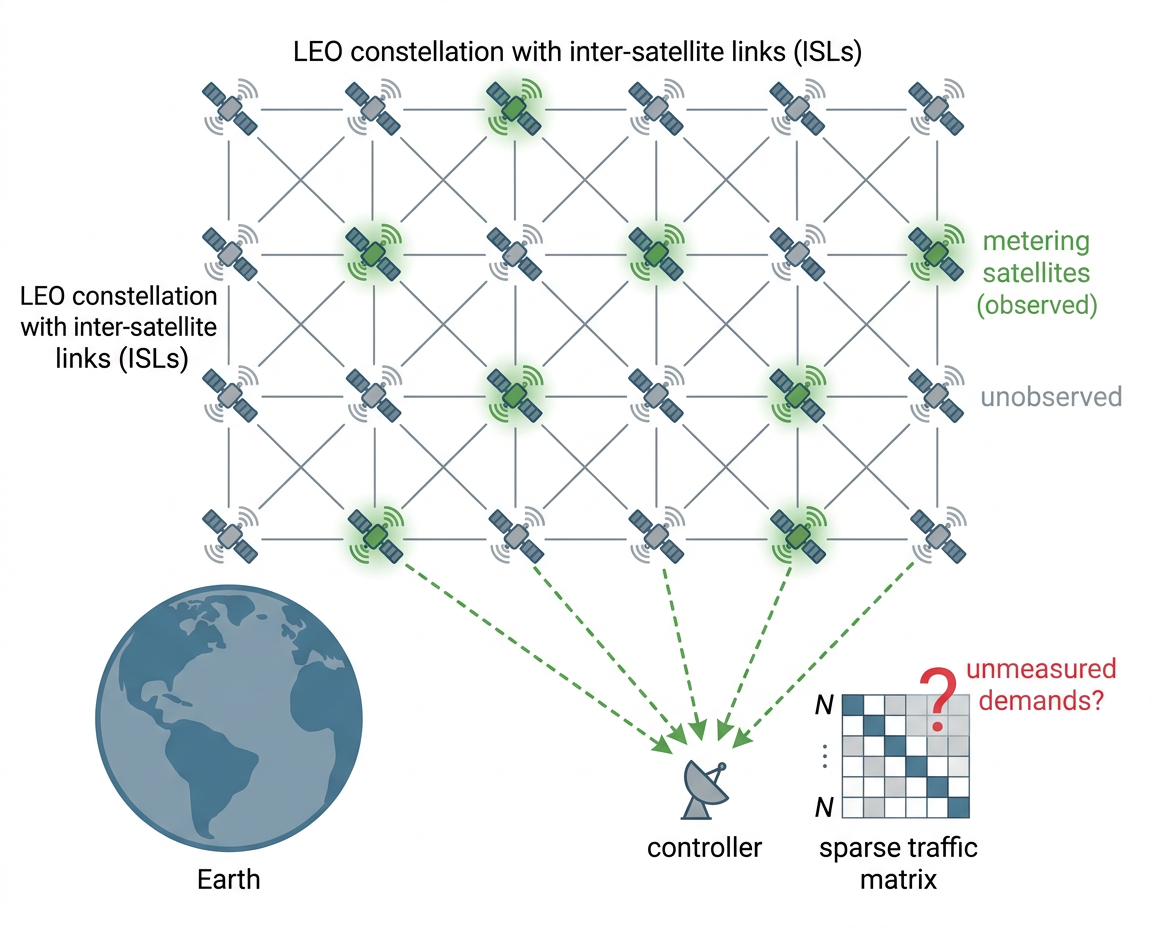
\includegraphics[width=\linewidth]{figures/scenario-draft.png}
    \caption{Sparse traffic observation in an LEO constellation. Only a
    subset of satellites meters traffic, so the controller receives a
    sparse traffic matrix while remaining responsible for all demands.}
    \label{fig:scenario}
\end{figure}

In LEO constellations, sparse observation interacts with geographic traffic
concentration and orbital motion in three ways. First, when metering is
available on only a subset of satellites, an unmeasured source hides a whole
row of demands, not just isolated matrix entries. Since satellites serving
populated footprints can carry substantial traffic~\cite{kassing2020},
zero filling may erase an entire source's contribution to ISL load; explicit
matrix completion instead risks passing reconstruction errors into routing~\cite{zhang2009}.
Second, traffic from nearby footprints shares multi-hop ISL corridors, while
satellite motion changes the association between ground users and ingress
satellites. The allocator must combine current path--link relationships with
recent traffic evolution without allowing imputed values to distort shared
link representations~\cite{t2gnn}. Third, moving footprints change the active
source--destination pairs as the constellation evolves. A model tied to a
fixed demand list would require resizing or retraining, despite the limited
onboard resources and short control windows~\cite{sate}. These coupled
measurement and mobility constraints distinguish sparse-observation TE in
LEO constellations from the static terrestrial setting~\cite{test}.

We present \sysname{} (\underline{Spa}rse-aware \underline{T}raffic
\underline{E}ngineering), a learned allocator designed around these
constraints. It represents each unobserved demand with a learnable mask
embedding rather than a fabricated volume. A mask-gated flow-centric graph
neural network (GNN) lets unobserved demands receive
link-state information without injecting their \emph{placeholders}, the
surrogate values that stand in for unmeasured demands at the model input,
into link embeddings. A temporal Transformer~\cite{vaswani2017} encodes
recent sparse observations, and per-demand cross-attention fuses temporal
and spatial evidence before predicting path split ratios. Shared weights
and demand pruning keep the model independent of the instantaneous demand
set, enabling reuse across constellation snapshots and scales.

After allocation, \sysname{} can optionally refine residual overloads using
link loads estimated from the same sparse observation. The important input
to this lightweight step is a neighbor estimate: an unmeasured demand is
inferred from observed demands sharing its source satellite. This estimate
uses geographic locality to avoid granting the controller an unavailable
ground-truth traffic matrix. It is an implementation aid to the sparse-aware
allocator rather than the organizing principle of the system.

We evaluate \sysname{} on a 1{,}584-satellite Starlink Shell-1
constellation over observation ratios from $2\%$ to $50\%$, measuring the
realized maximum link utilization (MLU) against ground-truth demands. Each
configuration is evaluated through repeated runs with matched random
initializations, separating observation-dependent effects from variation
between runs. \sysname{} holds the
realized MLU in the $1.64$--$1.89$ range, within $1.19$--$1.37\times$ of a
path-restricted LP optimum, while deciding in under $0.4$~s per snapshot and
transferring to a one-third-scale constellation without architectural change.
Against impute-then-optimize pipelines and zero-filled temporal baselines the
outcomes are mixed and no single pairwise comparison reaches significance; we
therefore examine the distributions across repeated runs to identify where
sparse-aware allocation helps and where simple fill-based treatments remain
competitive.

Our contributions are as follows:
\begin{itemize}
    \item We formulate sparse-observation TE for LEO constellations in which
    limited satellite telemetry leaves individual demands or entire source
    rows unmeasured. The formulation separates the controller's partial
    information from the true ISL loads used to evaluate its decisions.
    Predicting path split ratios allows routing decisions for unmeasured
    demands without requiring explicit recovery of their volumes.
    \item We design \sysname{} to combine the spatial structure of ISL routes
    with the recent evolution of geographically concentrated satellite traffic.
    Learnable mask embeddings distinguish missing measurements from zero
    traffic, asymmetric path--link propagation isolates those embeddings from
    measured link evidence, and cross-attention integrates the spatial features
    with sparse observation history. Demand pruning and shared parameters let
    the same architecture accommodate changing active pairs as satellite
    footprints move, without tying its weights to a fixed constellation graph.
    \item We evaluate \sysname{} on a 1{,}584-satellite constellation across
    $2\%$--$50\%$ observability, with a smaller same-family constellation as a
    scale check. Matched comparisons and ablations distinguish the effects of
    sparse-input representation, training, and observation-based refinement.
    The results identify observation-dependent performance and initialization
    sensitivity, bounding the conditions under which the proposed design
    improves MLU instead of assuming a uniform advantage.
\end{itemize}

The remainder of this paper is organized as follows.
\Cref{sec:related} reviews related work. \Cref{sec:formulation} formulates
the sparse-observation TE problem. \Cref{sec:design} presents \sysname{}.
\Cref{sec:eval} evaluates the system, and \cref{sec:conclusion} concludes
the paper.

\section{Related Work}
\label{sec:related}

% 迁移自 docs/related_work.md；bib 条目已全部核实（2026-08）。

\subsection{ML-Driven Traffic Engineering for WANs}

Traffic engineering has long been formulated as a constrained optimization
problem~\cite{fortz2000,wang2006} solved by linear programming (LP), whose
runtime scales poorly with network size. Kumar \emph{et al.} proposed
SMORE~\cite{smore}, which decouples robust oblivious path selection
from online rate adaptation, while Abuzaid \emph{et al.}~\cite{ncflow} and
Narayanan \emph{et al.}~\cite{pop} accelerate LP by problem decomposition,
trading allocation quality for speed. A recent line of work replaces online
solvers with learned models~\cite{valadarsky2017}: Perry \emph{et al.}
proposed DOTE~\cite{dote}, which directly maps historical traffic matrices to
split ratios with stochastic optimization; Xu \emph{et al.} proposed
Teal~\cite{teal}, combining a flow-centric graph neural network (GNN),
multi-agent reinforcement learning (RL), and alternating direction method of
multipliers (ADMM) fine-tuning to achieve near-optimal allocations with
orders-of-magnitude speedups; and Liu \emph{et al.} proposed
FIGRET~\cite{figret}, which enhances robustness against traffic uncertainty at
per-flow granularity. To survive topology changes without retraining, AlQiam
\emph{et al.} proposed HARP~\cite{harp}, enforcing invariances to node
permutation and tunnel reordering so that it transfers across topologies unseen
in training; Fan \emph{et al.} proposed Aether~\cite{aether2025}, pursuing the
same generality with elastic multi-agent graph transformers, and Ye
\emph{et al.}~\cite{ye2025} trained path-based GNNs for robust distributed TE
under link failures. More recently, Wu \emph{et al.}~\cite{netllm} explored
large language models as general-purpose traffic planners. However, all of
these systems assume the \emph{complete} traffic matrix is available at
decision time, an assumption that rarely holds in large-scale satellite
networks, where network-wide measurement is prohibitively expensive.

\subsection{TE and Routing for Satellite Networks}

LEO mega-constellations pose unique challenges for TE: topologies change
every few tens of milliseconds as satellites move, and control decisions
must be produced within stringent latency
budgets~\cite{handley2018,bhattacherjee2019,kassing2020}. Classical
approaches
absorb mobility through topology abstractions; the virtual node model of Lu
\emph{et al.}~\cite{vn2013} binds logical nodes to earth-fixed footprints so
that upper-layer routing observes a quasi-static grid. Optimization-based
satellite TE has explored segment routing~\cite{hu2022}, distributed
clustering that optimizes elephant flows separately~\cite{wei2024}, and
supervised learning for distributed split-ratio prediction~\cite{flexsate2024}.
Wu \emph{et al.} proposed SaTE~\cite{sate}, the
state-of-the-art learning-based TE for satellite constellations: it
formulates a heterogeneous graph over satellites, demands, paths, and links,
prunes zero-traffic relations to make training tractable on a single GPU,
and selects representative topologies via Graph2Vec and determinantal point
process (DPP) sampling so that
one trained model generalizes across topology snapshots with millisecond
inference. In parallel, Yang \emph{et al.} proposed FNC~\cite{fnc,fnc-infocom},
which targets dynamic traffic
allocation for earth-observation constellations, replacing RL with
end-to-end imitation learning and substituting iterative constraint solvers
with normalization-based feasibility layers. Notably, FNC's imitation
learning requires expert allocation labels computed from complete training
matrices. Our offline training also uses complete traffic to evaluate rewards,
but does not require expert allocation labels; the distinction is not the
availability of training-time ground truth. Both SaTE and FNC, like their WAN counterparts,
assume the traffic matrix is fully observable at decision time. Unlike SaTE
and FNC, \sysname{} performs TE from sparse observations, down to a $2\%$
observation ratio (\cref{tab:related}).

\subsection{TE with Incomplete Traffic Observations}

Network-wide traffic measurement is expensive: collecting a complete
traffic matrix requires instrumenting all ingress nodes at fine time
granularity, which is particularly onerous on resource-constrained
satellite platforms. A classical workaround is a two-stage pipeline:
first estimate or complete the traffic matrix via network tomography
(Vardi~\cite{vardi1996}; Zhang \emph{et al.}~\cite{zhang2003}), matrix
completion, or compressive sensing~\cite{zhang2009}, then optimize routing on
the estimate. However, reconstruction errors propagate to and degrade the
downstream allocation, since a single reconstructed matrix is handed to a
separate optimizer. Guo \emph{et al.} proposed TEST~\cite{test}, which, to
our knowledge, is the first \emph{end-to-end} approach to learn routing
policies directly from sparsely measured traffic matrices rather than first
reconstructing them; it integrates a Transformer over historical sparse
sequences with a graph convolutional network (GCN) over the topology, fills
unobserved entries with zeros, compensates with synthesized training
augmentation, and targets terrestrial networks with static topologies. In the
graph learning literature, Huo \emph{et al.}~\cite{t2gnn} addressed message
passing under missing node features via teacher-student distillation, but such
techniques have not been applied to network TE. No prior work, to our
knowledge, performs TE from sparse traffic observations in satellite networks,
where the difficulty is compounded by time-varying topologies and drifting
demand sets. Unlike TEST, which fills unobserved entries with zeros and
targets static terrestrial networks, \sysname{} replaces missing entries with
learnable mask embeddings, gates their message passing, and handles LEO
dynamics---time-varying topologies and drifting demand-pair sets---via demand
pruning with size-invariant weights, enabling train-once, zero-retraining
deployment; it further uses a source-neighbor estimate for optional
congestion-aware refinement without consulting the unobserved ground-truth
matrix (\cref{tab:related}).

\begin{table}[t]
    \caption{Comparison with the related works.}
    \label{tab:related}
    \centering
    \footnotesize
    \setlength{\tabcolsep}{3pt}
    \begin{tabular}{@{}lccccc@{}}
        \toprule
        & Teal~\cite{teal} & SaTE~\cite{sate} & TEST~\cite{test}
        & FNC~\cite{fnc} & \textbf{Ours} \\
        \midrule
        Satellite scenario      & \xmark & \cmark & \xmark & \cmark & \cmark \\
        Dynamic topology        & \xmark & \cmark & \xmark & \cmark & \cmark \\
        Sparse observation      & \xmark & \xmark & \cmark & \xmark & \cmark \\
        Temporal modeling       & \xmark & \xmark & \cmark & \xmark & \cmark \\
        Mask-aware model        & \xmark & \xmark & \xmark & \xmark & \cmark \\
        Neighbor estimate        & \xmark & \xmark & \xmark & \xmark & \cmark \\
        Demand-set drift        & \xmark & partial & \xmark & \xmark & \cmark \\
        \bottomrule
    \end{tabular}
\end{table}

\section{Model and Problem Formulation}
\label{sec:formulation}

% 迁移自 docs/formulation.md；符号修正已应用：候选路径数 kappa，demand 集合 \mathcal{K}^t

\subsection{Network and Traffic Model}
\label{sec:model}

We model the constellation at control epoch $t$ as a directed graph
$G^t = (V, E^t)$, where $V$ is the set of $N$ satellites and $E^t$ the set of
inter-satellite links (ISLs), each link $e$ with capacity $c_e$. Time is
slotted into control epochs; within an epoch the topology snapshot is fixed,
while across epochs both $E^t$ and the traffic change as satellites move.

Traffic is described by a demand matrix $D^t \in \mathbb{R}^{N \times N}$,
where $d_i$ denotes the volume of the $i$-th source-destination pair. Since
satellite traffic is geographically concentrated, we maintain an \emph{active
demand set} $\mathcal{K}^t$, the pairs with nonzero demand in recent
history, and only these are modeled. Each demand
$i \in \mathcal{K}^t$ is served by $\kappa$ pre-selected candidate paths
$P_i = \{p_{i,1}, \ldots, p_{i,\kappa}\}$ ($\kappa = 4$ edge-disjoint
shortest paths in our implementation). The TE decision for demand $i$ is a
split-ratio vector $r_i \in \mathbb{R}^{\kappa}$ with $r_{i,k} \ge 0$ and
$\sum_k r_{i,k} \le 1$, allocating flow $f_{i,k} = r_{i,k} \cdot d_i$ to path
$p_{i,k}$; the residual $1 - \sum_k r_{i,k}$ represents intentionally
unserved traffic. Main notations are summarized in \cref{tab:notation}.

\begin{table}[t]
    \caption{Main Notations.}
    \label{tab:notation}
    \centering
    \footnotesize
    \begin{tabular}{@{}ll@{}}
        \toprule
        Symbol & Definition \\
        \midrule
        $G^t=(V,E^t)$ & constellation graph at epoch $t$; $c_e$ link capacity \\
        $D^t$, $d_i$ & demand matrix; volume of demand $i$ \\
        $\mathcal{K}^t$ & active demand set at epoch $t$ \\
        $\kappa$, $P_i$ & candidate paths per demand; path set of demand $i$ \\
        $r_i$, $f_{i,k}$ & split ratios of demand $i$; flow on path $p_{i,k}$ \\
        $M$, $\rho$ & binary observation mask; observability ratio \\
        $O^t$, $H^t$ & sparse observation $D^t{\odot}M$; last-$L$ history \\
        $\phi$ & learnable mask embedding for unmeasured demands \\
        $A$, $\tilde{A}$ & bipartite adjacency; its mask-gated variant \\
        $H_S$, $H_T$, $H_F$ & spatial, temporal, and fused embeddings \\
        $\pi_\theta$, $R$ & TE policy network; ground-truth reward \\
        \bottomrule
    \end{tabular}
\end{table}

\subsection{TE with Complete Observation}
\label{sec:complete-te}

With the complete demand matrix available, TE is the classic path-based
allocation problem, for which two objectives dominate the literature.
\emph{Load balancing} minimizes the maximum link utilization (MLU),
the standard objective in satellite TE, where hot ISLs over populated
regions dictate quality of service~\cite{sate,hu2022,wei2024}:
\begin{align}
    \min_{\{r_{i,k}\}} \quad & \theta \label{eq:mlu} \\
    \text{s.t.} \quad
        & \frac{1}{c_e}\!\!\sum_{(i,k):\, e \in p_{i,k}}\!\! r_{i,k} d_i
          \le \theta,
        && \forall e \in E^t, \label{eq:mlu-cap} \\
        & \sum_{k=1}^{\kappa} r_{i,k} = 1,
        && \forall i \in \mathcal{K}^t, \label{eq:conserve} \\
        & r_{i,k} \ge 0,
        && \forall i, k, \label{eq:mlu-nonneg}
\end{align}
where \cref{eq:conserve} enforces flow conservation: every demand must
be fully served, so $\theta$ cannot be lowered by simply withholding
traffic. \emph{Throughput maximization} instead maximizes the total
satisfied demand, permitting demands to be served only partially when
capacity is scarce (total-flow TE~\cite{teal,ncflow}):
\begin{align}
    \max_{\{f_{i,k}\}} \quad
        & \sum_{i \in \mathcal{K}^t} \sum_{k=1}^{\kappa} f_{i,k}
        \label{eq:obj} \\
    \text{s.t.} \quad
        & \sum_{k=1}^{\kappa} f_{i,k} \le d_i,
        && \forall i \in \mathcal{K}^t, \label{eq:demand} \\
        & \sum_{(i,k):\, e \in p_{i,k}} f_{i,k} \le c_e,
        && \forall e \in E^t, \label{eq:capacity} \\
        & f_{i,k} \ge 0,
        && \forall i, k. \label{eq:nonneg}
\end{align}
Both problems are linear programs solvable to optimality, but at
constellation scale their solve time far exceeds the control
epoch~\cite{sate}. More fundamentally for this paper, the
link-load terms in \cref{eq:mlu-cap,eq:capacity}, as well
as the per-demand cap in \cref{eq:demand}, all require knowing $d_i$ for
\emph{every} active demand. We treat MLU minimization as the primary
objective throughout this paper, following the satellite TE literature,
and report throughput maximization as a secondary instantiation to show
that our design is objective-agnostic.

\subsection{TE with Sparse Observation}
\label{sec:sparse-te}

\subsubsection{Observation Model}
At each epoch only a subset of demands is measured. A binary mask
$M \in \{0,1\}^{|\mathcal{K}^t|}$ marks demand $i$ as measured ($M_i = 1$) or
not ($M_i = 0$), and the controller receives the sparse observation
\begin{equation}
    O^t = D^t \odot M, \quad \text{together with } M \text{ itself},
    \label{eq:obs}
\end{equation}
where $\odot$ is the element-wise product. \Cref{fig:sparse-tm} contrasts a
ground-truth traffic matrix from our Starlink trace with its node-level
sparse observation. We consider two measurement
granularities: \emph{flow-level}, where a fraction $\rho$ of demand pairs is
sampled, and \emph{node-level}, where a fraction $\rho$ of satellites meter
all their outgoing demands; the latter matches deployments where
measurement capability resides on a subset of satellites. The controller
additionally retains the last $L$ sparse observations
$H^t = (O^{t-L+1}, \ldots, O^t)$.

\begin{figure}[t]
    \centering
    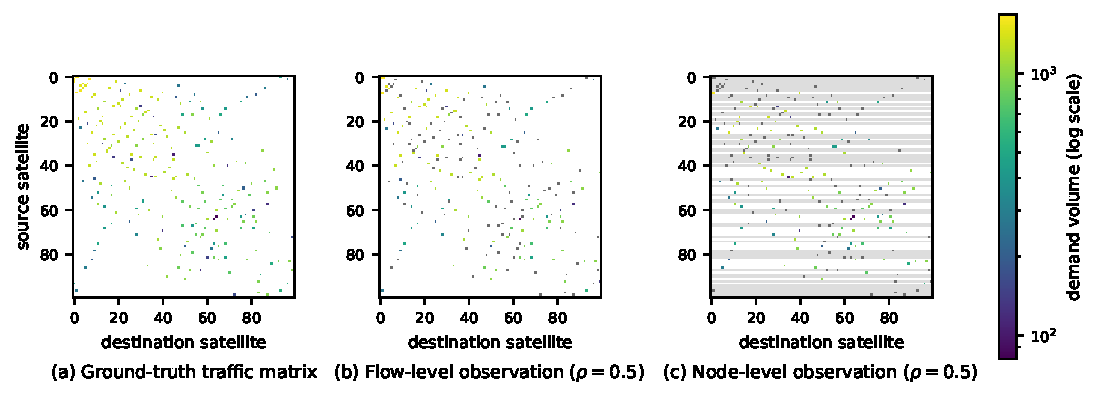
\includegraphics[width=\linewidth]{figures/sparse-tm.pdf}
    \caption{A ground-truth traffic matrix from the Starlink $22{\times}72$
    trace (150 busiest satellites shown) and its node-level sparse
    observation: white cells carry no traffic, gray rows are unmeasured
    source satellites, and colored cells are observed demands.}
    \label{fig:sparse-tm}
\end{figure}

\subsubsection{Problem Statement}
A key observation makes decision-making under unknown demands physically
executable: the decision variables are split \emph{ratios}, not absolute
volumes. Once installed in the forwarding plane, $r_i$ is applied
multiplicatively to whatever traffic actually arrives, so a decision for
demand $i$ requires no knowledge of $d_i$. Sparse-observation TE then
seeks a policy $\pi$ that maps the observable state to
split ratios for \emph{all} active demands,
\begin{equation}
    \{r_i\}_{i \in \mathcal{K}^t} = \pi\left(H^t, M, G^t\right),
    \label{eq:policy}
\end{equation}
maximizing the \emph{ground-truth} objective. Let
$f_{i,k}(\pi) = \tilde{r}_{i,k} \cdot d_i$ denote the flow actually
delivered on path $p_{i,k}$, where $\{\tilde{r}_i\}$ are the policy's
ratios after an optional repair step: ADMM
refinement with rounding under the throughput objective, and
conservation-preserving rebalancing under MLU, where the ratios are
already conservation-feasible by \cref{eq:conserve} but may still
overload individual links. Formally, for MLU minimization
\begin{equation}
    \min_{\pi} \;
    \mathbb{E}_t \Bigl[ \max_{e \in E^t}
        \frac{1}{c_e}\!\!\sum_{(i,k):\, e \in p_{i,k}}\!\! f_{i,k}(\pi)
    \Bigr],
    \label{eq:sparse-mlu}
\end{equation}
and, for the throughput variant,
\begin{equation}
    \max_{\pi} \;
    \mathbb{E}_t \Bigl[ \sum_{i \in \mathcal{K}^t} \sum_{k=1}^{\kappa}
        f_{i,k}(\pi) \Bigr],
    \label{eq:sparse-obj}
\end{equation}
where the expectations are over traffic and topology dynamics. Note that
the link loads in \cref{eq:sparse-mlu} are evaluated with the true
demands $d_i$: an unmeasured demand still consumes real capacity even
though the policy could not see it, so misjudging it inflates the
realized MLU. The problem
is a partially observable sequential decision problem: unlike
\crefrange{eq:mlu}{eq:nonneg}, where the same $D^t$ appears in both
the decision and the constraints, here the decision variables and the
evaluation live in different information sets: the policy acts on
$(O, M)$ only, while feasibility and performance are settled by the
hidden $D$. Intuitively, the policy is graded against an exam it never
gets to read in full.

\subsection{Solution Paradigm}
\label{sec:paradigm}

Three solution families exist for \cref{eq:sparse-mlu,eq:sparse-obj}.
\emph{Solve-with-zeros} plugs $O$ directly into the
LP in \crefrange{eq:mlu}{eq:nonneg}, implicitly assuming unmeasured
demands are zero; the resulting policy leaves no headroom on the links
that unmeasured traffic actually traverses, so the realized MLU can be far
above the optimum (and, under the throughput objective, unmeasured
demands are structurally starved). \emph{Two-stage} approaches first estimate $\hat{D}$ from $(H, M)$,
via interpolation, tensor completion, or compressive
sensing~\cite{vardi1996,zhang2003,zhang2009}, and then
solve the LP on $\hat{D}$; estimation is optimized for reconstruction error,
which is misaligned with allocation quality, and errors propagate un-damped
into the allocation. We instead adopt \emph{end-to-end learning}:
parameterize $\pi_\theta$ as a neural network and optimize $\theta$ directly
against the TE objective,
\begin{equation}
    \max_{\theta} \;
    \mathbb{E} \bigl[ R\bigl(\pi_\theta(H, M, G),\, D\bigr) \bigr],
    \label{eq:rl-obj}
\end{equation}
where $R$ is the TE objective evaluated on the true $D$: negative
realized MLU for \cref{eq:sparse-mlu}, or total satisfied demand
for \cref{eq:sparse-obj}. Since $R$
is non-differentiable through the capacity-constrained network and the true
$D$ is available only as a training-time signal, we
optimize \cref{eq:rl-obj} with multi-agent reinforcement learning, in
which each demand acts as an agent sharing $\theta$ and receives a
COMA-style marginal-contribution reward, followed by an
optional lightweight repair step at inference that relieves overloaded
links. This paradigm makes the observation
model in \cref{eq:obs} a property of the \emph{input}, and the optimization
target in \cref{eq:sparse-obj} a property of the \emph{training signal},
cleanly separating what the policy can see from what it is optimized for.

\section{\sysname{} Design}
\label{sec:design}

% 迁移来源：docs/design.md（4.1 按批注瘦身为 pipeline 总览 + 引用 §III）

\subsection{Overview}
% [TODO] pipeline 总览一段 + Figure~\ref{fig:arch}（架构图：稀疏 TM+mask →
% 掩码嵌入 → 门控 GNN ↔ 时序编码 → 交叉注意力融合 → per-demand policy → ADMM），
% formulation 细节引用 \cref{sec:formulation

% \begin{figure}[t] ... \label{fig:arch}

\subsection{Mask-Aware Demand Representation}
% [TODO] 迁移 4.2：可学习掩码嵌入 $\theta$；卖点句 trained under the TE
% objective, not a reconstruction loss；T2-GNN~\cite{t2gnn} 先例

\subsection{Gated Message Passing}
% [TODO] 迁移 4.3：非对称门控 $\tilde{A}$；listeners 比喻；零参数零开销

\subsection{Temporal-Spatial Fusion}
% [TODO] 迁移 4.4：Transformer 时序编码（log 压缩稳定性）+ per-demand
% 交叉注意力；[XX] ms 待回填

\subsection{Scaling to Dynamic Constellations}
% [TODO] 迁移 4.5：demand 剪枝（2.5M→6.3K，SaTE~\cite{sate} 同源）+ 零重训
% （runtime inputs, not parameters）+ 路径模板 + 最短路兜底

\subsection{Training and Constraint Repair}
% [TODO] 迁移 4.6：COMA MARL（复用 Teal~\cite{teal}）；双轨句；
% RL vs IL~\cite{fnc} 防守点；ADMM 修复

\section{Evaluation}
\label{sec:eval}

% 评估章节：Setup → 整体对比 → 稀疏感知分配器隔离实验 →
% 邻居估算敏感性 → 跨规模 → 延迟 → takeaways。

\subsection{Setup}
\label{sec:setup}

\textbf{Constellation.} Our main testbed is a Starlink Shell-1 Walker
constellation~\cite{giuliari2020} interconnected in a $+$Grid pattern
(\cref{tab:constellation}); orbital dynamics are derived from the
Satellite Tool Kit (STK). With 1{,}584 satellites, an average path length
of 23.51 hops, and a diameter of 47, capacity conflicts between demands
are far more frequent than in the terrestrial WANs used in prior TE
studies~\cite{teal}. For the cross-scale check
(\cref{sec:cross-scale}) we use a one-third-scale instance of the same
architecture (24 planes $\times$ 22 satellites, 528 nodes).

\begin{table}[t]
    \caption{Simulation parameters of the Starlink constellation.}
    \label{tab:constellation}
    \centering
    \footnotesize
    \begin{tabular}{@{}ll@{}}
        \toprule
        Parameter & Value \\
        \midrule
        Height of LEO satellites & 550 km \\
        Constellation configuration & Walker \\
        Total number of satellites & 1{,}584 \\
        Number of orbital planes & 72 \\
        Satellites per plane & 22 \\
        Inclination of orbits & $55^{\circ}$ \\
        Phase factor & 3 \\
        Inter-satellite links & 6{,}336 \\
        \bottomrule
    \end{tabular}
\end{table}

\textbf{Traffic.} Traffic matrices are generated by random city
sampling~\cite{giuliari2021}: cities are drawn with probability
proportional to their population, each sampled city pair is attached to
its nearest satellites, and per-pair flows are aggregated into
satellite-level demands (\cref{tab:tm-stats}). We use 101 consecutive
snapshots (one every 5 minutes), with snapshots 0--79 for training,
80--89 for validation, and 90--100 for testing, a strict temporal
split with no leakage. Under the chosen ISL capacities, a path-restricted
LP with complete traffic information attains a mean MLU of
${\approx}1.38$ on the test snapshots. The main setting therefore tests load
balancing under overload, not guaranteed capacity-feasible delivery;
\cref{sec:complete-te} defines the meaning of MLU above one. Demand pruning (\cref{sec:scaling})
restricts the modeled
demand set to the ${\sim}6.3$K pairs that ever carry traffic, out of
2.5M node pairs.

\begin{table}[t]
    \caption{Statistics of the population-based traffic trace (Mbps).}
    \label{tab:tm-stats}
    \centering
    \footnotesize
    \setlength{\tabcolsep}{4pt}
    \begin{tabular}{@{}lc@{}}
        \toprule
        Metric & Value \\
        \midrule
        Snapshots (5-min interval) & 101 \\
        Nonzero demand, max & 1{,}800 \\
        Nonzero demand, mean$\pm$std & 159.5 $\pm$ 242.3 \\
        Total demand per snapshot & 890{,}242 \\
        Active pairs per snapshot & 5{,}583 \\
        Active-pair union (trace) & 6{,}334 \\
        \bottomrule
    \end{tabular}
\end{table}

\textbf{Metric and protocol.} Our metric is the \emph{realized MLU}
evaluated against ground-truth demands (lower is better); flow
conservation in \cref{eq:conserve} is enforced by construction, so MLU
cannot be gamed by under-serving traffic. We sweep the observation
ratio $\rho \in \{0.02, 0.05, 0.1, 0.3, 0.5\}$ and use five independent
experimental repeats per configuration, controlled by random seeds
0--4. Matching repeat indices use the same seed across methods. Unless
stated otherwise, every method is paired with the \emph{identical deployable
post-processing layer}: two rounds of ten rebalancing sweeps, whose
utilization estimate reads only the sparse observation with neighbor fill
(\textsc{obs-nbr}, \cref{sec:training}),
so that no method receives unavailable demand information and the
allocator remains the only factor that varies. The \textsc{oracle} variant,
which reads the ground-truth matrix, appears only in the neighbor-estimation
diagnostic. Each plotted point is the mean MLU over the same eleven
chronological test snapshots for one experimental repeat. We show all five
repeats and summarize them by mean$\pm$standard deviation, median, and range.
Because the snapshots in a trace are temporally correlated, headline
comparisons are paired on $(\rho,\text{repeat})$, not on snapshots, and are
assessed with two-sided sign tests.

\textbf{Baselines.} All learned baselines share the training pipeline,
path sets, and optional neighbor-assisted refinement of \sysname{} and differ
only in how they handle sparsity:
\begin{itemize}
    \item \emph{zero-fill}: the sparse adaptation of full-observation
    systems such as Teal~\cite{teal} and SaTE~\cite{sate}, which
    cannot run on an incomplete matrix; unobserved entries are set to
    zero and the model is trained end to end on the filled input.
    SaTE's heterogeneous-graph allocator targets the same
    MLU objective with the same pruning, so this variant is its
    closest sparse-input proxy.
    \item \emph{mean-interp}: a two-stage complete-then-optimize
    baseline that fills unobserved entries with the mean of observed
    demands before allocation.
    \item \emph{nbr-fill}: a stronger two-stage baseline that fills
    each unobserved demand from observed demands sharing its source
    satellite, the same estimate used by the optional refinement.
    \item \emph{TEST-inspired}: a controlled baseline motivated by
    TEST~\cite{test}, with zero-filled input, a Transformer over the
    observation history ($L=3$), and an ungated GCN. We use the same paths,
    objective, and training pipeline as the other methods rather than
    claiming reproduction of TEST's original terrestrial setup.
    \item \emph{untrained}: the \sysname{} architecture with weights
    frozen at random initialization, isolating the contribution of
    training. It is \emph{not} the LP optimum: the LP (\cref{eq:mlu}) needs
    the complete matrix and serves only as a full-information lower-bound
    reference for MLU (${\approx}1.38$), not as an online sparse-input baseline.
\end{itemize}

\begin{table}[t]
    \caption{Model and training hyperparameters (defaults held fixed
    across all $\rho$ and repeats).}
    \label{tab:hparams}
    \centering
    \footnotesize
    \setlength{\tabcolsep}{4pt}
    \begin{tabular}{@{}ll@{}}
        \toprule
        Parameter & Value \\
        \midrule
        FlowGNN layers $\Lambda$ & 6 \\
        Candidate paths $\kappa$ & 4 \\
        Temporal $d_{\mathrm{model}}$ / heads / layers & 16 / 2 / 1 \\
        Fusion dim $d_{\mathrm{fuse}}$ & 8 \\
        History length $L$ & 3 \\
        COMA samples per update & 30 \\
        Mask-embedding init & 57.0 (median nonzero demand) \\
        \midrule
        Learning rate & $1\!\times\!10^{-4}$ \\
        Epochs (warmup / early stop) & 60 (4 / on) \\
        Restart screening & 3 inits \\
        Batch size & 20 \\
        Untrained control & 0 epochs, 1 init \\
        Neighbor refinement (deployed) & 2 rounds $\times$ 10 sweeps \\
        \midrule
        Trainable parameters & 4{,}468 \\
        \bottomrule
    \end{tabular}
\end{table}

\textbf{Implementation.} \Cref{tab:hparams} lists the
hyperparameters, drawn from the code defaults and held fixed across all
$\rho$ and repeats. The untrained control shares the trained model's
random initialization and differs only in skipping gradient updates
(\texttt{epochs${=}0$}); it is therefore a clean ablation of the
\emph{training} factor with identical architecture, mask embedding, and
post-processing.

\subsection{Performance of \sysname{}}
\label{sec:own-results}

Across observation ratios from $2\%$ to $50\%$, \sysname{} achieves a
mean realized MLU in the $1.64$--$1.89$ range (the \sysname{} row of
\cref{tab:overall}), tightening as more demands become visible: from $1.885$
at $\rho=0.05$ down to $1.639$ at $\rho=0.5$. To calibrate these numbers we
solve a path-restricted LP that sees the \emph{complete} matrix on the same
test snapshots and candidate paths; it attains a full-information optimum of
MLU~${\approx}1.38$. Observing only a fraction of demands, \sysname{} stays
within $1.19$--$1.37\times$ of this optimum. An MLU of $1.7$ means that the
assigned load on the busiest link is $70\%$ above its capacity. Flow
conservation is maintained, but capacity feasibility is not: the metric
does not imply that all offered traffic is delivered within the epoch.
These overloaded-load-balancing results cannot establish delay, loss, or
admission-control guarantees. The full-observation LP provides a lower bound
on achievable MLU for the chosen paths, not an online sparse-input baseline;
it is distinct from the \emph{untrained} control, which uses random weights.

\subsubsection{Inference latency}
\label{sec:runtime}
On the 1{,}584-satellite constellation, one complete allocation pass
(demand-set assembly, graph rebuild, gated GNN, temporal encoder, fusion,
policy head, and optional neighbor-assisted refinement) completes in under
$0.4$~s per snapshot on a single GPU, against a 5-minute control period.
Combined with the $O(D)$ complexity of \cref{sec:complexity} and the
4{,}468-parameter model size, \sysname{} fits the compute envelope of a
constellation controller.

\subsubsection{Cross-scale generality}
\label{sec:cross-scale}
To test whether the allocator depends on constellation scale, we reuse its
size-invariant architecture on a one-third-scale Shell-1 instance with 528
satellites and 2{,}112 ISLs. \Cref{tab:cross-scale} isolates the learned
allocation prior without post-processing at two observation ratios. At
$\rho=0.05$, training lowers median MLU from $4.02$ to $3.04$ and improves all
three matched repeats. The result at $\rho=0.3$ is mixed, indicating that the
most informative observation regime shifts with traffic density. The model
requires no architectural change as the graph and demand-set sizes change,
which supports reuse across constellation scales while avoiding a claim of
uniform gains.

\begin{table}[t]
    \caption{Cross-scale check on the 528-satellite instance without
    post-processing (median MLU and paired training gain over three repeats).}
    \label{tab:cross-scale}
    \centering
    \footnotesize
    \setlength{\tabcolsep}{4pt}
    \begin{tabular}{@{}lcccc@{}}
        \toprule
        $\rho$ & Trained & Untrained & Paired gain & \sysname{} lower \\
        \midrule
        0.3  & 3.69 & 3.83 & $-3.2\%$  & 1/3 \\
        0.05 & 3.04 & 4.02 & $+24.4\%$ & 3/3 \\
        \bottomrule
    \end{tabular}
\end{table}

\subsection{Comparison with Sparsity Treatments}
\label{sec:overall}

We now compare \sysname{} against external sparsity treatments under the
identical deployable protocol. \Cref{fig:overall-distribution} shows all
150 results from repeated runs, while \cref{tab:overall} gives their numerical
summary. No method has a uniform advantage across observation ratios. In
particular, \sysname{} attains a lower MLU than zero filling on 16 of the 25
matched $(\rho,\text{repeat})$ pairs, but the paired sign test gives
$p=0.2295$; its comparisons with TEST-inspired, mean-interp, nbr-fill, and
untrained controls are likewise non-significant (\cref{tab:paired}). Hence
the observed rankings must be interpreted together with their variability;
they do not establish overall superiority.

\begin{figure*}[t]
    \centering
    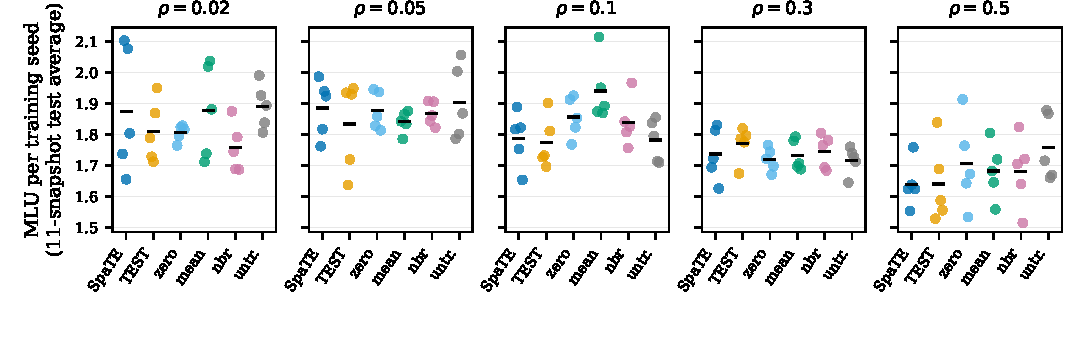
\includegraphics[width=\textwidth]{figs/overall_distribution.pdf}
    \caption{External comparison across five experimental repeats under
    the same deployed neighbor-assisted refinement. Each marker is one
    repeat's average MLU over
    the 11 test snapshots; black bars mark means. The dispersion explains why
    column-wise rankings based only on a median are not reliable evidence of
    a general advantage.}
    \label{fig:overall-distribution}
\end{figure*}

\begin{table*}[t]
    \caption{External comparison under the aligned deployable protocol.
    Entries are mean$\pm$standard deviation across five experimental repeats;
    medians and ranges are included in the supplementary CSV. Lower MLU is
    better.}
    \label{tab:overall}
    \centering
    \scriptsize
    \setlength{\tabcolsep}{5pt}
    \begin{tabular}{@{}lccccc@{}}
        \toprule
        & \multicolumn{5}{c}{observation ratio $\rho$} \\
        \cmidrule(lr){2-6}
        Method & 0.02 & 0.05 & 0.1 & 0.3 & 0.5 \\
        \midrule
        \sysname{} & $1.874\pm0.203$ & $1.885\pm0.093$ & $1.786\pm0.089$ & $1.737\pm0.085$ & $1.639\pm0.074$ \\
        TEST-inspired~\cite{test} & $1.809\pm0.100$ & $1.833\pm0.145$ & $1.773\pm0.083$ & $1.769\pm0.056$ & $1.639\pm0.127$ \\
        zero-fill~\cite{teal,sate} & $1.805\pm0.026$ & $1.876\pm0.061$ & $1.856\pm0.065$ & $1.719\pm0.038$ & $1.705\pm0.142$ \\
        mean-interp & $1.877\pm0.152$ & $1.840\pm0.035$ & $1.939\pm0.103$ & $1.732\pm0.050$ & $1.682\pm0.091$ \\
        nbr-fill & $1.756\pm0.079$ & $1.867\pm0.038$ & $1.839\pm0.078$ & $1.745\pm0.054$ & $1.680\pm0.114$ \\
        untrained & $1.890\pm0.073$ & $1.902\pm0.121$ & $1.781\pm0.068$ & $1.716\pm0.044$ & $1.757\pm0.107$ \\
        \bottomrule
    \end{tabular}
\end{table*}

\begin{table}[t]
    \caption{Paired comparison of \sysname{} against each external control
    over 25 $(\rho,\text{repeat})$ pairs. The middle column counts the pairs in
    which \sysname{} attains the lower MLU (out of 25); there are no ties.
    $p$ is a two-sided sign test.}
    \label{tab:paired}
    \centering
    \footnotesize
    \setlength{\tabcolsep}{4pt}
    \begin{tabular}{@{}lcc@{}}
        \toprule
        Control & \sysname{} lower / 25 & $p$ \\
        \midrule
        TEST-inspired & 11 & 0.6900 \\
        zero-fill & 16 & 0.2295 \\
        mean-interp & 16 & 0.2295 \\
        nbr-fill & 15 & 0.4244 \\
        untrained & 14 & 0.6900 \\
        \bottomrule
    \end{tabular}
\end{table}

\subsection{Ablations}
\label{sec:allocator-isolation}

\subsubsection{Effect of training}
We isolate the contribution of training by comparing \sysname{} with its
untrained counterpart under the common neighbor-assisted refinement.
\Cref{fig:internal-training} plots the five test averages for each condition,
one per experimental repeat.
Training attains the lower MLU in 14 of the 25 matched $(\rho,\text{repeat})$
pairs and the higher in 11, with no ties (two-sided sign test $p=0.690$). At
$\rho=0.5$, for example, the mean is $1.639\pm0.074$ after training versus
$1.757\pm0.107$ without training; at the other ratios the paired outcomes are
mixed. Thus these data do not establish a statistically significant
end-to-end training advantage, but they expose the initialization sensitivity that a
single aggregate score would hide.

\begin{figure*}[t]
    \centering
    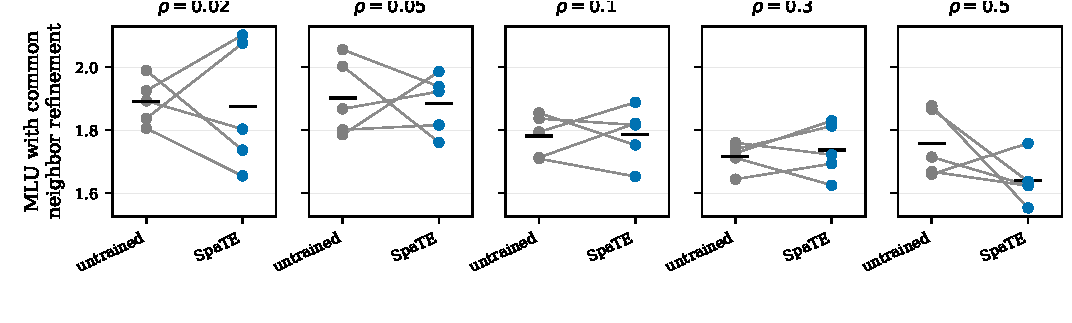
\includegraphics[width=\textwidth]{figs/internal_training.pdf}
    \caption{Effect of training under identical neighbor-assisted refinement.
    Gray dots denote the untrained control and blue dots denote \sysname{}.
    Each dot is one repeat's mean MLU over the same 11 test snapshots; slight
    horizontal offsets distinguish the five repeats, and black bars mark
    their means. Matching repeats share a random seed; no connecting lines
    are drawn.}
    \label{fig:internal-training}
\end{figure*}

\subsubsection{Representation components}
We next test the three representation choices without post-processing at the
two sparsest ratios, where their effect is least likely to be hidden by
rebalancing. \Cref{fig:component-lowrho} shows each experimental repeat. The
outcomes are mixed: no configuration dominates the others at both ratios,
and the three-repeat diagnostic is insufficient for a component-level
performance claim. We therefore retain the placeholder-isolation result of
\cref{prop:isolation} as a structural property, rather than interpreting it
as proof that gating, masking, or temporal encoding always lowers MLU.

\begin{figure*}[t]
    \centering
    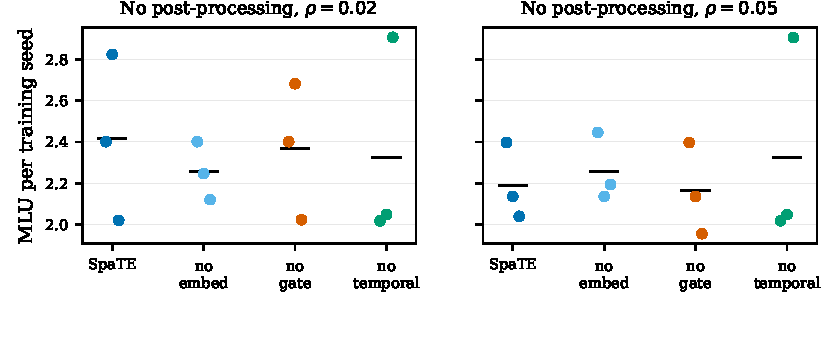
\includegraphics[width=0.76\textwidth]{figs/component_lowrho.pdf}
    \caption{Low-observability component diagnostic without post-processing
    (three experimental repeats). Dots are test averages from individual
    repeats and black bars are means. The mixed ordering supports treating
    the module choices as design alternatives rather than assuming a uniform
    component gain.}
    \label{fig:component-lowrho}
\end{figure*}

\subsubsection{Sensitivity to the neighbor estimate}
\label{sec:neighbor-estimate}
The optional refinement pass needs an estimated traffic matrix only to rank
candidate paths by congestion. \Cref{fig:neighbor-ladder} fixes the
untrained control at $\rho=0.3$ and shows all three experimental repeats.
Moving from no post-processing (median $2.833$) to an observation with zeros
elsewhere ($2.295$), and then to the source-neighbor estimate ($1.740$),
substantially changes the congestion signal available to the rebalancer. The
oracle reference reaches $1.599$, but uses unavailable ground-truth traffic
and five rounds of ten sweeps; it is a full-information diagnostic rather
than a protocol-matched baseline. The deployable conclusion is therefore limited to the value of the
neighbor estimate over zero filling, not a claim that post-processing is the
central learned mechanism.

\begin{figure}[t]
    \centering
    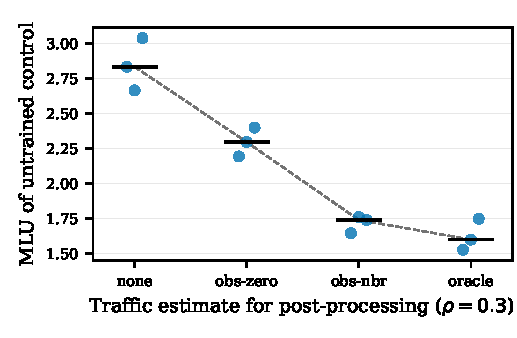
\includegraphics[width=\linewidth]{figs/neighbor_ladder.pdf}
    \caption{Sensitivity to the traffic estimate used by post-processing at
    $\rho=0.3$. Each dot is one experimental repeat; black bars denote medians.
    The oracle uses unavailable complete traffic and five rounds of ten
    sweeps; deployed methods use an observation-derived estimate.}
    \label{fig:neighbor-ladder}
\end{figure}

\subsection{Takeaways}
\label{sec:takeaways}

\begin{itemize}
    \item The distribution across experimental repeats, not a column-wise
    median, is required to interpret sparse-observation TE: none of \sysname{}'s
    external pairwise comparisons is statistically significant.
    \item Training and the three representation choices show mixed outcomes
    in the available internal diagnostics; the architecture's structural
    properties should not be read as a universal performance guarantee.
    \item Source-neighbor estimation provides a substantially more useful
    deployable congestion signal than zero filling in the $\rho=0.3$
    diagnostic, while the oracle remains an unavailable reference.
\end{itemize}

\section{Conclusion}
\label{sec:conclusion}

This paper studied MLU-oriented traffic engineering for LEO satellite
constellations when telemetry constraints expose only a small fraction of
demands. We presented \sysname{}, a sparse-aware learned allocator that
represents missing measurements explicitly, prevents placeholder traffic
from contaminating graph messages, and combines spatial and temporal
evidence before predicting path split ratios. Shared parameters and demand
pruning keep the architecture independent of the instantaneous demand-set
size.

Repeated evaluations on a 1{,}584-satellite Starlink constellation show
that MLU rankings vary with both the observation ratio and model
initialization.
\sysname{} attains the lower MLU on more matched trials than the zero-fill,
mean-interp, and nbr-fill controls, yet none of its external pairwise
comparisons is statistically significant. The component diagnostic is also
mixed at the two sparsest ratios. These negative results matter: they show
that the structural plausibility of a sparse-aware representation does not
by itself establish a uniform end-to-end MLU gain, and that comparisons
must account for variation across experimental repeats rather than rely on
a single summary statistic.

For deployment, a source-neighbor estimate can provide optional
post-processing with a useful congestion signal without access to the
complete traffic matrix. It is a supporting mechanism, not a substitute for
the sparse-aware allocator. Future work should improve robustness across
initializations and observation masks through adaptive measurement
scheduling, observation-aware model selection, and objectives that
explicitly control worst-case MLU.


\bibliographystyle{IEEEtran}
\bibliography{refs}

\end{document}
